%! Author = mr
%! Date = 6/1/25
\section{Entropic Swirl Gravity: Verlinde\rqs s Holography in a Topological Æther}

The Vortex Æther Model (VAM) describes spacetime and field interactions as manifestations of knotted vortex structures and swirl flow in a superfluid-like substrate. To bridge this model with information-theoretic gravity, we reinterpret the work of Verlinde \cite{Verlinde2011,Verlinde2016} within the VAM framework.

\begin{figure}[h!]
\centering
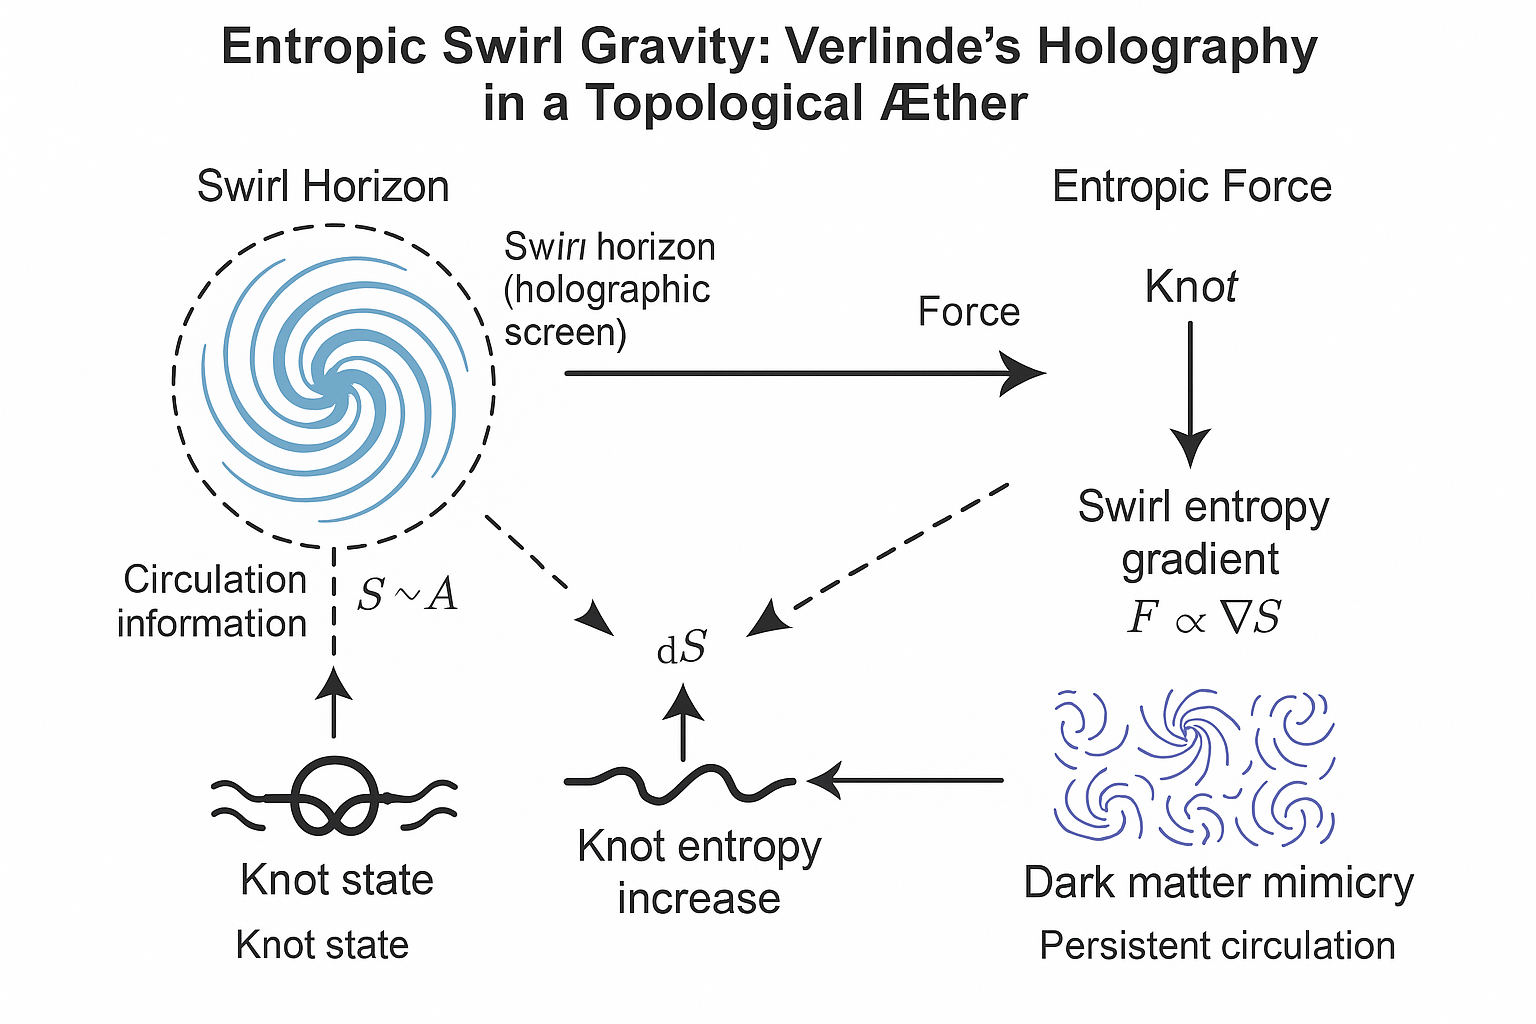
\includegraphics[width=0.65\textwidth]{images/ErikVerlinde}
\caption{Entropic Swirl Gravity in the Vortex Æther Model.
Swirl horizons in the æther act as holographic information surfaces, storing topological microstates of knotted vortex structures. Entropic gradients in swirl complexity generate emergent forces on probe knots, analogous to gravity in Verlinde\rqs s entropic framework. Large-scale coherent helicity fields can mimic dark matter halos by resisting entropy diffusion.}
\end{figure}

\subsection*{Gravity from Swirl Entropy Gradients}

Verlinde proposes that gravity is not a fundamental force but an emergent entropic effect arising from the statistical behavior of microscopic degrees of freedom. In VAM, these degrees of freedom are topological microstates—characterized by knot class, twist $T$, chirality $C$, and linking number $Lk$. Their configuration space defines a local entropy:
\begin{equation}
S_{\text{swirl}}(x) = k_B \log \Omega_{\text{topo}}(x),
\end{equation}
where $\Omega_{\text{topo}}$ is the number of accessible vortex configurations at position $x$. An entropy gradient results in a net force on test knots, analogous to an entropic force:
\begin{equation}
F_i = T \, \partial_i S_{\text{swirl}}.
\end{equation}
Here, $T$ is a notional temperature of the æther's microstates—interpreted as an effective \grqq twist activity\textquotedblright or reconnection rate.

\subsection*{Holography and Swirl Surfaces}

Verlinde incorporates the holographic principle: information within a volume is stored on its boundary surface. In VAM, the natural analog is a **swirl envelope**—a closed surface enclosing circulation density or knotted cores. The entropy of this envelope scales with area, not volume:
\begin{equation}
S_{\text{holo}} \propto A_{\text{swirl}}.
\end{equation}
These boundaries act as information horizons, and forces acting on test particles arise from changes in information across such surfaces.

\subsection*{Connection to Entropic Gravity}

The Vortex Æther Model (VAM) offers a mechanical realization of several core concepts in emergent gravity, as proposed by Verlinde~\cite{verlinde2017emergent}. In Verlinde\rqs s framework, gravitational attraction is not a fundamental force but arises from entropic gradients—information imbalances on holographic screens that encode microscopic degrees of freedom. Similarly, in VAM, gravity emerges from gradients in local swirl complexity: regions of higher vorticity act as information sinks, slowing down internal clock rates and drawing nearby topological structures inward.

The role of the holographic screen in Verlinde\rqs s theory is played in VAM by the \emph{swirl horizon}—a critical boundary beyond which the angular frequency $\omega_\text{obs}$ vanishes. These horizons trap information in topological cores, creating gradients in æther entropy that produce attractive forces. Additionally, the "elastic memory" of the æther in VAM provides a natural analog to Verlinde\rqs s emergent dark gravity: global tensions in the swirl field store energy in a nonlocal, long-range fashion without invoking dark matter particles.

Thus, VAM not only aligns with Verlinde\rqs s entropic hypothesis but provides a concrete fluid-dynamical model that grounds entropic force emergence in topological circulation states and observable time dilation effects.


\subsection*{Dark Matter as Topological Memory}

In Verlinde\rqs s emergent gravity model, apparent dark matter effects arise not from unseen mass but from the displacement of information across large entropy gradients \cite{Verlinde2016}. In VAM, this is interpreted as coherent swirl structures on galactic scales—regions with conserved or slowly diffusing helicity:
\begin{itemize}
    \item Galactic rotation curves arise from residual swirl tension.
    \item Topological inertia prevents decay of swirl gradients, mimicking \grqq phantom mass.\textquotedblright
    \item Threshold accelerations below a critical scale $a_0$ correspond to regions with degenerate knot microstates.
\end{itemize}

\subsection*{Entropic Time Flow and Geometrization}

Verlinde\rqs s model hints at spacetime geometry as an emergent, coarse-grained limit. In VAM, time flow itself is derived from swirl geometry:
\begin{equation}
d\tau \propto \vec{v} \cdot \vec{\omega},
\end{equation}
where $\vec{v}$ is the local swirl velocity and $\vec{\omega} = \nabla \times \vec{v}$ is the vorticity. This geometric definition of time ties directly into entropy production and circulation preservation. In effect:
\[
\text{Swirl = Spacetime}, \quad \text{Helicity = Entropy Flux}.
\]

\subsection*{Summary}

Verlinde\rqs s vision of gravity as an emergent, entropic phenomenon aligns naturally with the VAM picture:
\begin{itemize}
    \item Entropy is stored in swirl topologies;
    \item Forces emerge from gradients in circulation complexity;
    \item Spacetime geometry results from statistical distributions of vortex structures;
    \item Dark matter effects arise from preserved large-scale swirl modes.
\end{itemize}
Thus, VAM provides a physical substrate—absent in Verlinde\rqs s original proposal—capable of encoding entropy, information, and emergent gravitational phenomena through fluid-topological mechanisms.

